\documentclass[tikz,border=25pt]{standalone}
\usepackage[utf8]{inputenc}
\usepackage{xcolor}
\usepackage{tikz}
\usetikzlibrary{shapes.multipart, positioning, calc, arrows.meta}

% ==========================================
% Color Palette (Modern Slate & Accent Theme)
% ==========================================
\definecolor{tableheader}{RGB}{30, 41, 59}        % Slate 800
\definecolor{tableheadertext}{RGB}{255, 255, 255} % White
\definecolor{tablebody}{RGB}{248, 250, 252}       % Slate 50
\definecolor{tableborder}{RGB}{148, 163, 184}     % Slate 400
\definecolor{pkcolor}{RGB}{180, 83, 9}            % Amber 700
\definecolor{fkcolor}{RGB}{2, 132, 199}           % Sky 600
\definecolor{typecolor}{RGB}{100, 116, 139}       % Slate 500
\definecolor{linecolor}{RGB}{51, 65, 85}          % Slate 700
\definecolor{enumheader}{RGB}{79, 70, 229}        % Indigo 600
\definecolor{titlecolor}{RGB}{15, 23, 42}         % Slate 900

% ==========================================
% TikZ Styles
% ==========================================
\tikzset{
    table/.style={
        rectangle split,
        rectangle split parts=2,
        rectangle split part fill={tableheader, tablebody},
        rounded corners=3pt,
        draw=tableborder,
        line width=0.9pt,
        font=\small\ttfamily,
        align=left,
        inner sep=7pt
    },
    enumbox/.style={
        rectangle split,
        rectangle split parts=2,
        rectangle split part fill={enumheader, tablebody},
        rounded corners=3pt,
        draw=tableborder,
        line width=0.9pt,
        font=\footnotesize\ttfamily,
        align=left,
        inner sep=6pt
    },
    relation/.style={
        draw=linecolor,
        line width=1.1pt,
        -{Latex[length=2.8mm, width=2.2mm]}
    },
    cardinality/.style={
        font=\scriptsize\sffamily\bfseries,
        text=linecolor,
        inner sep=2pt
    }
}

\begin{document}
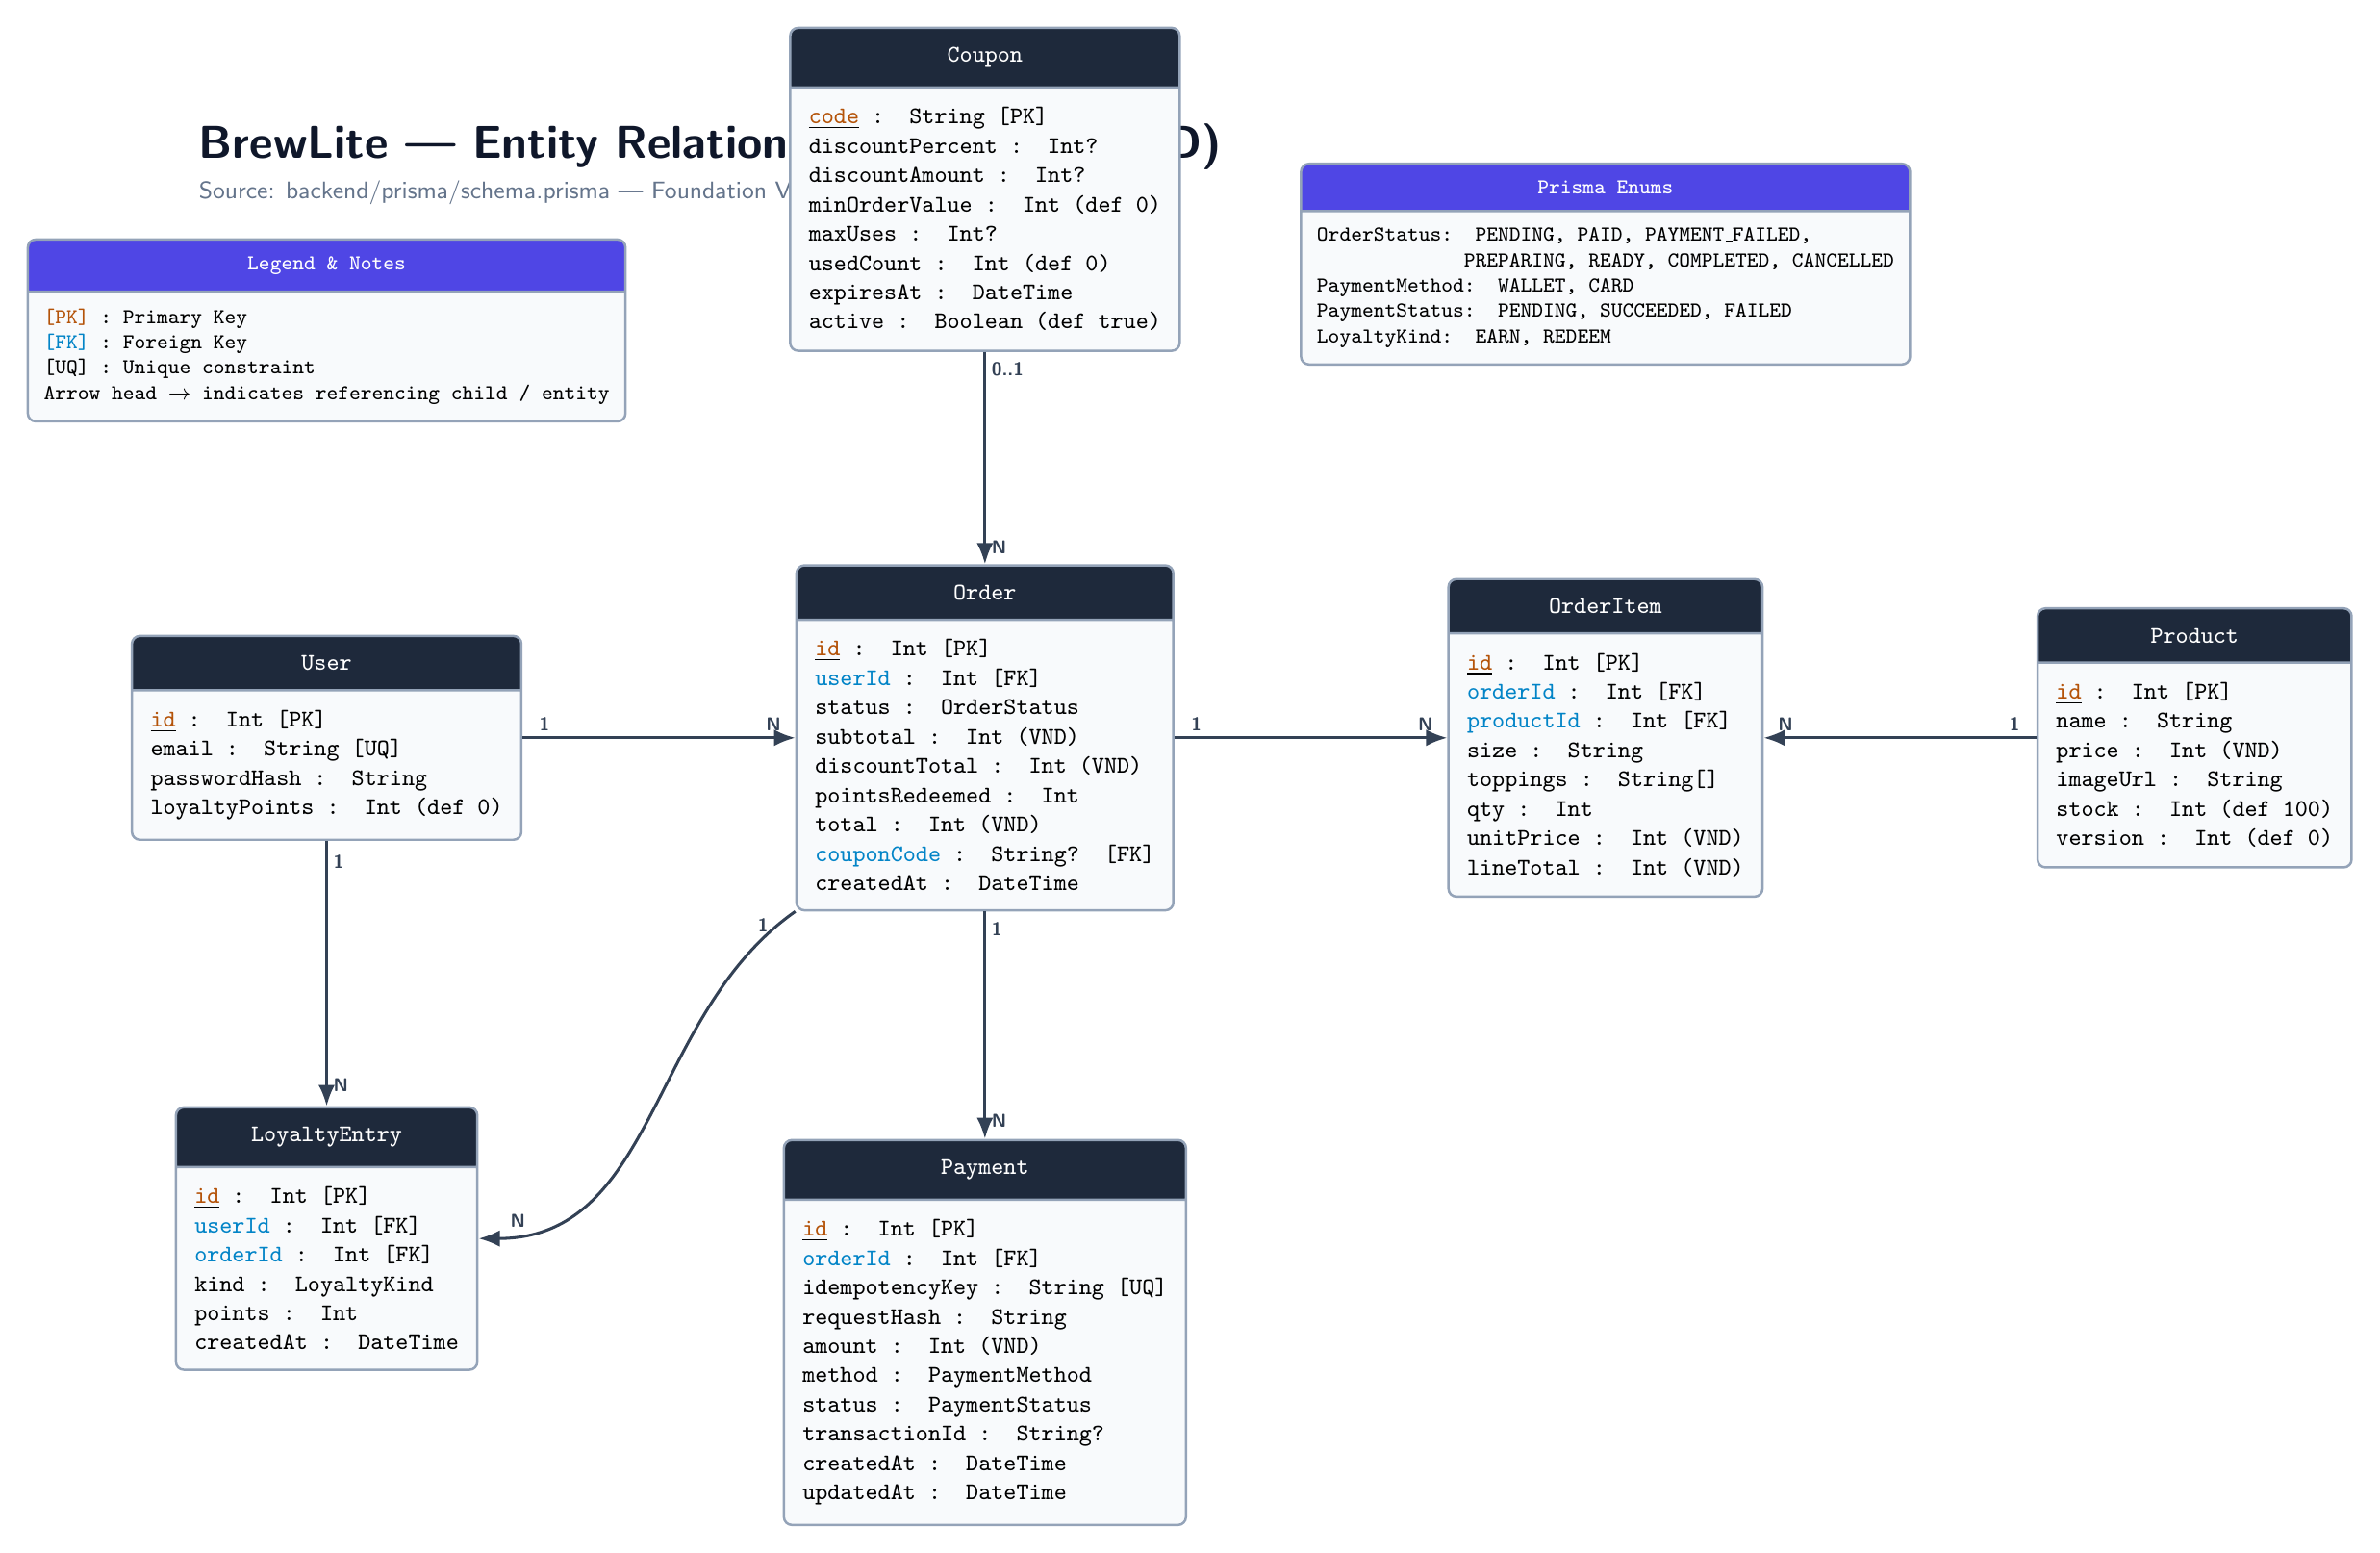
\begin{tikzpicture}[node distance=2.4cm and 3.2cm]

    % Diagram Title
    \node[anchor=west, font=\LARGE\bfseries\sffamily, text=titlecolor] at (-10.5, 7.8) {BrewLite --- Entity Relationship Diagram (ERD)};
    \node[anchor=west, font=\small\sffamily, text=typecolor] at (-10.5, 7.2) {Source: backend/prisma/schema.prisma | Foundation V1};

    % ------------------------------------------
    % Entities Definition
    % ------------------------------------------

    % Entity: Order (Center Pivot)
    \node[table] (order) at (0, 0) {
        \textbf{\textcolor{tableheadertext}{Order}}
        \nodepart{two}
        \underline{\textcolor{pkcolor}{id}} : Int \textbf{[PK]} \\
        \textcolor{fkcolor}{userId} : Int \textbf{[FK]} \\
        status : OrderStatus \\
        subtotal : Int (VND) \\
        discountTotal : Int (VND) \\
        pointsRedeemed : Int \\
        total : Int (VND) \\
        \textcolor{fkcolor}{couponCode} : String? \textbf{[FK]} \\
        createdAt : DateTime
    };

    % Entity: User (Left of Order)
    \node[table, left=3.6cm of order] (user) {
        \textbf{\textcolor{tableheadertext}{User}}
        \nodepart{two}
        \underline{\textcolor{pkcolor}{id}} : Int \textbf{[PK]} \\
        email : String \textbf{[UQ]} \\
        passwordHash : String \\
        loyaltyPoints : Int (def 0)
    };

    % Entity: OrderItem (Right of Order)
    \node[table, right=3.6cm of order] (orderitem) {
        \textbf{\textcolor{tableheadertext}{OrderItem}}
        \nodepart{two}
        \underline{\textcolor{pkcolor}{id}} : Int \textbf{[PK]} \\
        \textcolor{fkcolor}{orderId} : Int \textbf{[FK]} \\
        \textcolor{fkcolor}{productId} : Int \textbf{[FK]} \\
        size : String \\
        toppings : String[] \\
        qty : Int \\
        unitPrice : Int (VND) \\
        lineTotal : Int (VND)
    };

    % Entity: Product (Right of OrderItem)
    \node[table, right=3.6cm of orderitem] (product) {
        \textbf{\textcolor{tableheadertext}{Product}}
        \nodepart{two}
        \underline{\textcolor{pkcolor}{id}} : Int \textbf{[PK]} \\
        name : String \\
        price : Int (VND) \\
        imageUrl : String \\
        stock : Int (def 100) \\
        version : Int (def 0)
    };

    % Entity: Coupon (Above Order)
    \node[table, above=2.8cm of order] (coupon) {
        \textbf{\textcolor{tableheadertext}{Coupon}}
        \nodepart{two}
        \underline{\textcolor{pkcolor}{code}} : String \textbf{[PK]} \\
        discountPercent : Int? \\
        discountAmount : Int? \\
        minOrderValue : Int (def 0) \\
        maxUses : Int? \\
        usedCount : Int (def 0) \\
        expiresAt : DateTime \\
        active : Boolean (def true)
    };

    % Entity: Payment (Below Order)
    \node[table, below=3.0cm of order] (payment) {
        \textbf{\textcolor{tableheadertext}{Payment}}
        \nodepart{two}
        \underline{\textcolor{pkcolor}{id}} : Int \textbf{[PK]} \\
        \textcolor{fkcolor}{orderId} : Int \textbf{[FK]} \\
        idempotencyKey : String \textbf{[UQ]} \\
        requestHash : String \\
        amount : Int (VND) \\
        method : PaymentMethod \\
        status : PaymentStatus \\
        transactionId : String? \\
        createdAt : DateTime \\
        updatedAt : DateTime
    };

    % Entity: LoyaltyEntry (Below User)
    \node[table, below=3.5cm of user] (loyalty) {
        \textbf{\textcolor{tableheadertext}{LoyaltyEntry}}
        \nodepart{two}
        \underline{\textcolor{pkcolor}{id}} : Int \textbf{[PK]} \\
        \textcolor{fkcolor}{userId} : Int \textbf{[FK]} \\
        \textcolor{fkcolor}{orderId} : Int \textbf{[FK]} \\
        kind : LoyaltyKind \\
        points : Int \\
        createdAt : DateTime
    };

    % Enums & Legends Box
    \node[enumbox, above=2.8cm of orderitem] (enums) {
        \textbf{\textcolor{tableheadertext}{Prisma Enums}}
        \nodepart{two}
        \textbf{OrderStatus}: PENDING, PAID, PAYMENT\_FAILED, \\
        \phantom{\textbf{OrderStatus}:} PREPARING, READY, COMPLETED, CANCELLED \\
        \textbf{PaymentMethod}: WALLET, CARD \\
        \textbf{PaymentStatus}: PENDING, SUCCEEDED, FAILED \\
        \textbf{LoyaltyKind}: EARN, REDEEM
    };

    % Legend Box (Above User)
    \node[enumbox, above=2.8cm of user] (legend) {
        \textbf{\textcolor{tableheadertext}{Legend \& Notes}}
        \nodepart{two}
        \textcolor{pkcolor}{\textbf{[PK]}} : Primary Key \\
        \textcolor{fkcolor}{\textbf{[FK]}} : Foreign Key \\
        \textbf{[UQ]} : Unique constraint \\
        Arrow head $\rightarrow$ indicates referencing child / entity
    };

    % ------------------------------------------
    % Relationships / Foreign Key Connectors
    % ------------------------------------------

    % 1. User -> Order (1 : N)
    \draw[relation] (user.east) -- 
        node[cardinality, above, pos=0.08] {1} 
        node[cardinality, above, pos=0.92] {N} 
        (order.west);

    % 2. Order -> OrderItem (1 : N)
    \draw[relation] (order.east) -- 
        node[cardinality, above, pos=0.08] {1} 
        node[cardinality, above, pos=0.92] {N} 
        (orderitem.west);

    % 3. Product -> OrderItem (1 : N)
    \draw[relation] (product.west) -- 
        node[cardinality, above, pos=0.08] {1} 
        node[cardinality, above, pos=0.92] {N} 
        (orderitem.east);

    % 4. Coupon -> Order (0..1 : N)
    \draw[relation] (coupon.south) -- 
        node[cardinality, right, pos=0.08] {0..1} 
        node[cardinality, right, pos=0.92] {N} 
        (order.north);

    % 5. Order -> Payment (1 : N)
    \draw[relation] (order.south) -- 
        node[cardinality, right, pos=0.08] {1} 
        node[cardinality, right, pos=0.92] {N} 
        (payment.north);

    % 6. User -> LoyaltyEntry (1 : N)
    \draw[relation] (user.south) -- 
        node[cardinality, right, pos=0.08] {1} 
        node[cardinality, right, pos=0.92] {N} 
        (loyalty.north);

    % 7. Order -> LoyaltyEntry (1 : N)
    \draw[relation] (order.south west) to[out=215, in=0] 
        node[cardinality, above, pos=0.08] {1} 
        node[cardinality, above, pos=0.92] {N} 
        (loyalty.east);

\end{tikzpicture}
\end{document}
